\section{Versuchsaufbau}
\label{sec:Versuchsaufbau}

Dieser Versuch wird mit einer Apparatur, wie sie in 
Abbildung \ref{abb1} dargestellt ist, durchgeführt.
Dabei befindet sich eine Spektrallampe mit dem Material 
Cadmium (Cd) zwischen den Polen eines Elektromagneten, 
welche ein Magnetfeld erzeugen können, dessen Feldlinien 
transversal zu den elektromagnetischen Strahlen der 
Cd-Lampe verlaufen.
Ihr emittiertes Licht wird daraufhin durch ein Objektiv und 
eine Kondensorlinse auf einen Spalt gerichtet. Eine zweite 
Linse projeziert den Strahl danach auf ein Geradsichtprisma, 
welches die Eigenschaft hat, Licht nach seiner 
Wellenlänge separieren zu können. Jetzt kann es durch einen 
Polarisationsfilter nach seiner Polarisation und durch einen 
Spalt nach seiner Wellenlänge ausgewählt werden, sodass es 
schließlich auf eine Lummer-Gehrke-Platte \ref{LGP} abgebildet 
wird. Um eine vollständige Abbildung auf das Eintrittsfenster
der Platte und auf den davor verbauten Spalt zu ermöglichen, 
befinden sich zwischen Filter und Spalt, sowie zwischen 
Spalt und Lummer-Gehrke-Platte zwei weitere Linsen. 
Die Srahlen, die das Gehäuse um die Platte verlassen,
können schließlich mit einer Digitalkamera fotographisch 
festgehalten werden.

\begin{figure}
    \centering
    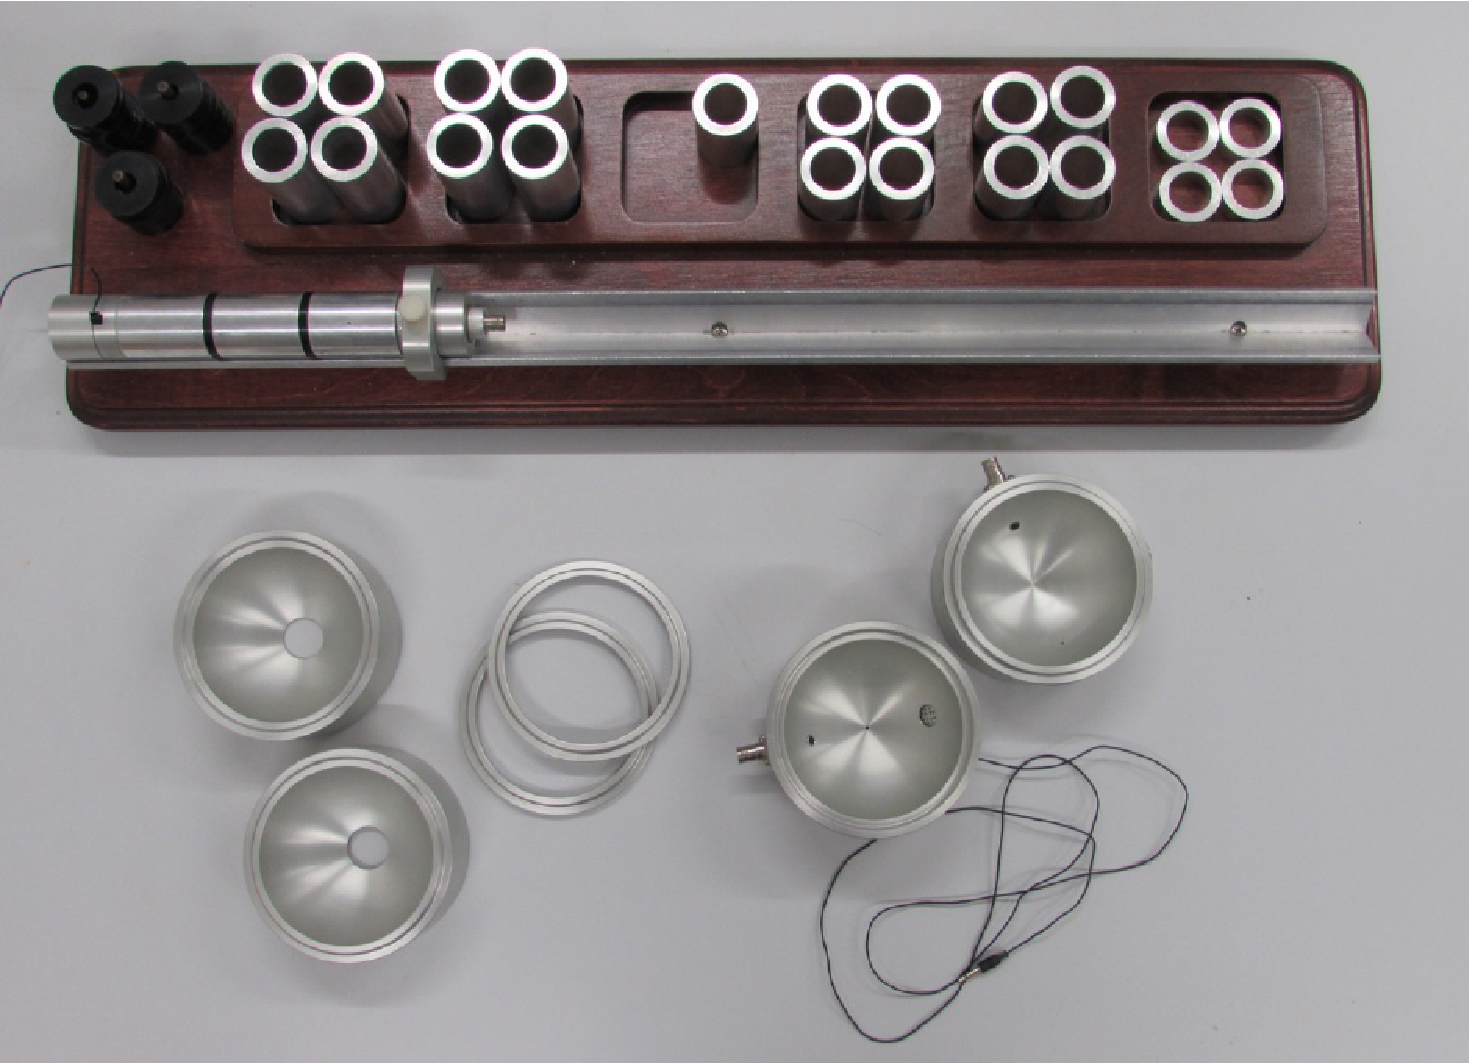
\includegraphics[width=\textwidth]{figure/Aufbau.pdf}
    \caption{Diese Abbildung zweigt den schematischen Aufbau dieses Versuches \cite{sample}.}
    \label{abb1}
\end{figure}

\subsection{Die Lummer-Gehrke-Platte}
\label{LGP}

Eine Lummer-Gehrke-Platte besteht aus zwei planparallelen 
Platten, welche im Abstand $d$ voneinander befestigt sind.
Am Eintrittsfenster in den durch die Platten begrenzten Raum 
befindet sich ein Prisma. Parallel einfallendes Licht kann 
wird durch das Prisma im Winkel $\beta$ auf eine der Platten 
gelenkt und an ihr reflektiert, sodass es im glaichen Winkel 
auf die andere Platte treffen kann. Auf diese Weise durchläuft 
ein Lichtstrahl die Lummer-Gehrke-Platte, wobei immer auch
ein Teil an den Reflektionspunkten im Winkel $\alpha$ transmittiert wird. 
Zwischen den Transmissionsstrahlen herrscht genau dann 
konstruktive Interferenz wenn die Bedingung

\begin{equation}
    2nd \cos(\beta) = m \lambda
    \label{eq1}
\end{equation}

gilt. $\lambda$ ist in dieser Gleichung die Wellenlänge des 
einfalllenden Lichtstrahles und $n$ der Brechungsindex der Platte, 
welcher durch 

\begin{equation}
    n = \frac{\sin(\alpha)}{\sin{\beta}}
    \label{eq2}
\end{equation}

gegeben ist. Einen weiteren EInfluss hat die Ordnungszahl der 
Interferenz, welche in Gleichung \ref{eq1} durch $m$
gegeben ist.\\
Für den Fall eines monochromatischen einfallenden 
Lichtstrahls ist der Gangunterschied der Interferenz von der
Breite der Wellenlänge des Lichtes. 
Das führt dazu, dass sich die Änderung der Wellenlänge an der 
Änderung des Abstandes des Interferezstreifen ablesen lässt.
Eine solche Änderung kann bspw. durch ein eingeschaltetes 
Magnetfeld am Elektromagneten \ref{abb1} erzeugt werden.\\
Das DIsppersionsgebiet einer Lummer-Gehrke-Platte ist 
der Spektralbereich für den eine Messung möglich ist. 
Um eine Überlagerung der Ordnungen zu vermeiden, sollten 
zwei Wellenlängen maximal auf eine Differenz von der 
Größe dieses Spektralbereiches aufgespalten werden. 
Für große Austrittswinkel $\alpha$ ist er durch 

\begin{equation}
    \delta \lambda_{\symup{D}} = \frac{\lambda^2}{2d} \frac{1}{\sqrt{n^2 -1}}
    \label{eq:del_Lam}
\end{equation}

gegeben. Das Auflösungsvermögen einer Lummer-Gehrke-Platte ist 
neben ihr zugeordneten Eigenshcaften, wie der Plattenlänge und 
dem Brechungsindex, auch von der Wellenlänge des Lichtes 
abhängig. Es kann über den folgenden Zusammenhang bestimmt 
werden:

\begin{equation}
    A = \frac{\lambda}{\delta \lambda} = \frac{L}{\lambda}(n^2 -1)
    \label{eq:del_A}
\end{equation}

\section{Versuchsdurchführung}
\label{sec:Versuchsdurchführung}

